\documentclass[11pt]{article}

\usepackage{fontspec}
\usepackage[margin=1in]{geometry}
\usepackage{amsmath}
\usepackage{tikz}
\usepackage{authblk}
\usetikzlibrary{arrows.meta,positioning}
\usepackage[hidelinks]{hyperref}

\newcommand{\sha}{\operatorname{SHA256}}
\newcommand{\pTwoTR}{\operatorname{P2TR}}
\newcommand{\concat}{\mathbin\|}
\setlength{\emergencystretch}{2em}

\title{Decentralized Asset Management Protocol on \\
Liquid using Simplicity}
\author{Kyrylo Riabov, Artem Chystiakov}
\affil{Blockstream}
\date{\today}

\begin{document}

    \maketitle

    \begin{abstract}
        We propose a decentralized protocol for managing regulated Liquid assets.
        Unlike an offchain cosigning service, ordinary transfers require no issuer signature.
        A holder signs the spend of the asset and supplies a policy proof, enforced by the Simplicity covenant onchain in the same transaction.
        In case the issuer's service goes offline, holders who retained access to the latest policy snapshot can continue transacting under those rules.
        The design preserves holder custody and confines the asset to compliant covenants, still allowing the issuer to update the rules dynamically.
        The protocol supports mutable blacklists, whitelists, and transfer limits.
    \end{abstract}


    \section{Introduction}

    Liquid assets are native ledger assets with optional reissuance authority \cite{liquid,liquid-assets}.
    However, an issuer may still need to restrict their use.
    Common controls include sanctions, court-ordered freezes, account approval, and transaction limits.
    Circle (USDC) contracts include pause and blacklist roles \cite{usdc-contracts}.
    Tether (USDT) also states that it may freeze or burn tokens in specified circumstances \cite{tether-rid}.

    Blockstream AMP2 enforces issuer rules via a 2-of-2 wallet, with the user and the platform each holding one key.
    Every asset transfer requires a second signature from the platform \cite{liquid-assets}.
    This gives the issuer a simple enforcement point.
    However, it also makes transfer availability depend on the cosigning service being constantly online.

    We replace that with policy evaluation enforced fully onchain.
    An issuer posts a policy snapshot and commits to it in a Simplicity verifier covenant \cite{simplicity}.
    Any asset holder with the snapshot can construct the required proofs and initiate the transfer without the issuer's participation.
    In this paper, \emph{decentralized} describes transfer execution and policy data distribution.
    However, it does not describe policy governance -- the issuer still chooses and updates the rules.

    The protocol combines three ideas.
    A programmable signature authorizes the holder \cite{programmable-signatures}.
    A verifier output identifies the applicable rules.
    A confinement covenant returns every regulated output to the same ownership form.
    Sections~\ref{sec:model} and~\ref{sec:construction} introduce these ideas before giving their Taproot construction.
    Section~\ref{sec:policies} presents example policies.
    Section~\ref{sec:security} states the resulting guarantees and limits.


    \section{Protocol Model}
    \label{sec:model}

    \subsection{Assets and roles}

    The \emph{issuer} creates a regulated Liquid asset $A$ and controls an issuer key $I$.
    Liquid also allows the creation of reissuance tokens whose holders may mint more units of $A$ \cite{liquid-assets}.
    This authority is separate from the protocol.
    The issuer may destroy the reissuance token for a fixed supply of $A$ or retain it under its governance.
    Nevertheless, any later issuance must enter the regulated covenant.
    Otherwise the issuer has created unregulated units of $A$.

    The issuer also creates a distinct \emph{verifier asset} $V$.
    A valid verifier output carries a fixed amount $q$ of $V$.
    The issuer may destroy $V$'s reissuance token for a deployment with only one verifier output.
    It may instead retain this token and create more verifier outputs as demand grows -- this reduces contention and increases throughput.
    Each unspent verifier output $C_V(\pi)$ identifies the policy $\pi$ enforced on its spending path.

    A \emph{holder} controls an x-only public key $X$ and receives $A$ in a user covenant $C_U(X)$.
    A \emph{recipient} is simply the holder selected for a new output.
    The two covenants have different roles:

    \begin{itemize}
        \item $C_U(X)$ proves authorization by $X$ and requires the verifier output at transaction input zero.
        \item $C_V(\pi)$ enforces the current policy $\pi$ on its primary path and confines every new $A$ output to some $C_U(Y)$.
    \end{itemize}

    Thus neither program trusts the other as data.
    The same transaction joins them.
    The user covenant requires $q$ units of $V$.
    The verifier output can move on its primary path only by executing the verifier covenant.
    Coordination among several such outputs is outside this paper's scope.

    \subsection{Setup}

    The issuer performs four setup steps:

    \begin{enumerate}
        \item Issue $A$ and place its circulating supply in user covenants.
        \item Issue $q$ units of $V$ and choose whether to retain $V$'s reissuance authority.
        \item Choose an initial policy snapshot $D_{\pi_0}$ and publish enough data to reproduce the proofs.
        \item Lock these $q$ units of $V$ in the verifier covenant $C_V(\pi_0)$.
    \end{enumerate}

    The commitment $\pi_0$ authenticates $D_{\pi_0}$ but does not make the data available.
    Holders or independent mirrors must retain the full snapshot if they are willing to spend without the issuer's service.

    \subsection{Holder transfer}

    Suppose $X$ pays $Y$.
    The transaction spends $C_V(\pi)$ at input zero with one or more $C_U(X)$ inputs afterwards.
    Each user input requires its owner to provide a BIP-340 signature over Simplicity's \texttt{sig\_all\_hash} \cite{bip340,simplicity-sighash}, committing to the entire transaction.
    The design follows the programmable signature pattern described in the companion work \cite{programmable-signatures}.

    The verifier input then performs two tasks.
    First, it requires every output carrying $A$ to use the user covenant, where the intended recipient key becomes a parameter of that covenant.
    Second, the verifier evaluates the issuer's policy using transaction data and proofs supplied by the holder.
    The transaction is valid only if both the owner authorization and the verifier checks succeed.

    Figure~\ref{fig:transfer} shows the primary spending flow.
    Output zero recreates the same verifier covenant.
    Payments and change return to user covenants.

    \begin{figure}[ht]
        \centering
        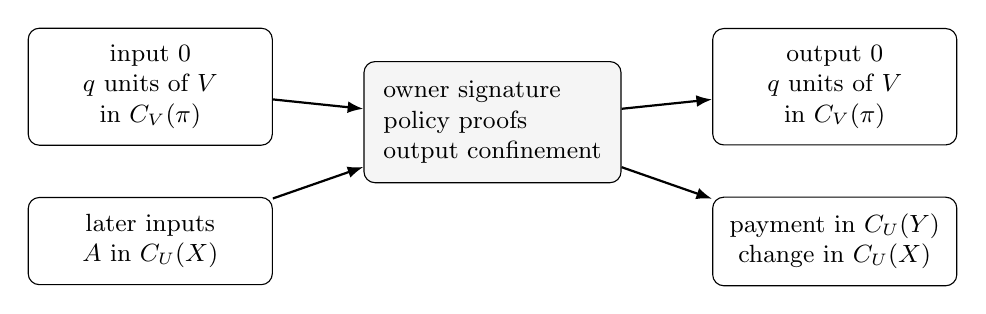
\begin{tikzpicture}[
            node distance=0.65cm and 1.15cm,
            box/.style={draw, rounded corners, align=center, font=\small, inner sep=6pt, minimum width=3.1cm},
            check/.style={draw, rounded corners, align=left, font=\small, inner sep=7pt, fill=black!4},
            arrow/.style={-{Latex[length=2mm]}, thick}
        ]
        \node[box] (vin) {input 0\\$q$ units of $V$\\in $C_V(\pi)$};
        \node[box, below=of vin] (ain) {later inputs\\$A$ in $C_U(X)$};
        \node[check, right=of vin, yshift=-0.45cm] (checks) {owner signature\\policy proofs\\output confinement};
        \node[box, right=of checks, yshift=0.45cm] (vout) {output 0\\$q$ units of $V$\\in $C_V(\pi)$};
        \node[box, below=of vout] (aout) {payment in $C_U(Y)$\\change in $C_U(X)$};

        \draw[arrow] (vin) -- (checks);
        \draw[arrow] (ain) -- (checks);
        \draw[arrow] (checks) -- (vout);
        \draw[arrow] (checks) -- (aout);
        \end{tikzpicture}
        \caption{An ordinary transfer. No issuer signature is required.}
        \label{fig:transfer}
    \end{figure}

    \subsection{Issuer update}

    The verifier output uses a NUMS internal key and has two script spending paths.
    The primary path enforces holder transfers and an issuer path verifies a signature under $I$ over the entire transaction.
    This allows the issuer to move $V$ to any successor script.
    They can use the secret key behind $I$ to move $V$ to $C_V(\pi')$, changing the policy commitments or the verifier logic.
    Additionally, the issuer path may also be used to halt all transfers by moving $V$ elsewhere.
    No hidden Taproot leaf stores separate policy state.
    Instead, $\pi$ is a parameter of the primary path verifier program and the resulting TapLeaf hash $P(\pi)$ commits to that policy.
    Hence, the locking script $C_V(\pi)$ also commits to the same policy.
    The issuer spends the old verifier output through the issuer path.
    It then creates a successor locked to $C_V(\pi')$ and sets the primary path of the successor script to use $\pi'$.

    This authority does not reveal a holder key and it does not satisfy a user covenant.
    The issuer alone therefore cannot spend a holder's balance.
    It can only change the rules for future transfers authorized by holders.


    \section{Covenant Construction}
    \label{sec:construction}

    \subsection{User covenant state}

    We use the Taproot state construction from the Simplicity documentation \cite{simplicity-state,bip341}.
    Let $U$ be the Elements TapLeaf hash of the fixed Simplicity user program.
    Let $K$ be a NUMS internal key.
    For a tag $t$, define the tagged hash as
    \begin{equation}
        H_t(m)=\sha\bigl(\sha(t)\concat\sha(t)\concat m\bigr).
    \end{equation}
    For an owner key $X$, define
    \begin{align}
        D(X) &= H_{\mathtt{TapData}}(X), \\
        B(a,b) &= H_{\mathtt{TapBranch/elements}}
        \bigl(\min(a,b)\concat\max(a,b)\bigr), \\
        R_U(X) &= B\bigl(U,D(X)\bigr), \\
        C_U(X) &= \pTwoTR\bigl(K,R_U(X)\bigr).
    \end{align}
    Here $\pTwoTR(K,r)$ is the Elements Taproot locking script obtained by tweaking internal key $K$ with script root $r$.
    Elements uses its own tagged hash domains for Taproot \cite{elements-taproot}.

    Figure~\ref{fig:user-tree} contains one executable leaf and one unspendable \texttt{TapData} leaf.
    Changing $X$ changes the output without changing the program $U$.
    This lets the verifier covenant embed $U$ and derive a recipient covenant from a supplied public key.

    \begin{figure}[ht]
        \centering
        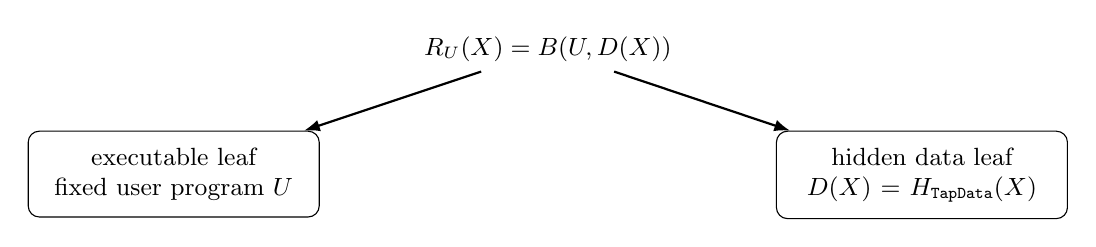
\begin{tikzpicture}[
            node distance=0.75cm and 1.2cm,
            root/.style={font=\small},
            box/.style={draw, rounded corners, align=center, font=\small, inner sep=6pt, text width=0.27\linewidth},
            arrow/.style={-{Latex[length=2mm]}, thick}
        ]
        \node[root] (root) {$R_U(X)=B(U,D(X))$};
        \node[box, below left=of root] (exec) {executable leaf\\fixed user program $U$};
        \node[box, below right=of root] (state) {hidden data leaf\\$D(X)=H_{\mathtt{TapData}}(X)$};
        \draw[arrow] (root) -- (exec);
        \draw[arrow] (root) -- (state);
        \end{tikzpicture}
        \caption{Only the user covenant carries hidden Taproot state.}
        \label{fig:user-tree}
    \end{figure}

    \subsection{User authorization}

    To spend $C_U(X)$ through $U$, the witness reveals $X$ and a signature $\sigma_X$.
    The Simplicity program recomputes $C_U(X)$ and compares it with its current locking script.
    A witness therefore cannot substitute another key.
    The program then checks
    \begin{equation}
        \operatorname{BIP340Verify}\bigl(X,\operatorname{sigAllHash}(T),\sigma_X\bigr)=1,
    \end{equation}
    where $T$ is the spending transaction.
    The program also checks three facts.
    Its current input must contain explicit asset $A$.
    This input cannot be zero.
    Input zero must contain explicit verifier asset $V$ in amount $q$.

    These checks establish custody -- they do not duplicate policy logic.
    Policy is enforced when the same transaction spends a verifier output.

    \subsection{Verifier covenant}

    Let $P(\pi)$ be the primary spending path of the Simplicity verifier program instantiated with policy commitment $\pi$.
    Let $G(I)$ be the issuer spending path.
    This path requires a BIP-340 signature under $I$ over \texttt{sig\_all\_hash} and allows any successor script for $V$.
    Using the NUMS internal key $K$, define
    \begin{align}
        R_V(\pi) &= CommitmentMerkleRoot\bigl(P(\pi),G(I)\bigr), \\
        C_V(\pi) &= \pTwoTR\bigl(K,D(R_V(\pi))\bigr).
    \end{align}
    Spending through $P(\pi)$ is the primary transfer path.
    Spending through $G(I)$ is the issuer update path.
    The NUMS key provides no key path spend.

    On the primary path, $P(\pi)$ performs the following checks:

    \begin{enumerate}
        \item Its input is transaction input zero and contains $q$ units of $V$.
        \item Output zero returns $q$ units of $V$ to the same $C_V(\pi)$.
        \item At least one regulated input is a $C_U(X)$ input. This input independently requires its owner signature. Only holders can therefore advance the verifier output.
        \item Every output exposes its asset identifier. Every input and output of $A$ exposes a positive amount, and the verifier requires the two explicit totals to be equal. Every output of $A$ has locking script $C_U(Y)$ for its supplied recipient key $Y$.
        \item All enabled policy predicates hold.
    \end{enumerate}

    The output scan advances until the transaction has no output at the next index.
    A confidential asset commitment would hide which outputs need confinement. Hence, asset identifiers must be explicit.
    The v0.1 verifier also makes regulated values explicit and checks their exact input/output sum. This keeps the amount invariant independently auditable inside the covenant instead of relying on caller metadata or implicit transaction inference.

    The fixed-index input may be functionally limiting.
    The research of an arbitrary-index positioning is considered future work.

    \subsection{State transitions}

    An ordinary transfer has the abstract form
    \begin{align}
        T_{\mathrm{in}} &=[(V,q,C_V(\pi)),(A,a_1,C_U(X_1)),\ldots], \\
        T_{\mathrm{out}}&=[(V,q,C_V(\pi)),(A,b_1,C_U(Y_1)),\ldots,\mathrm{fees}].
    \end{align}
    Every user input supplies its owner signature, and the verifier input supplies the policy proofs.
    Liquid's asset conservation and the two covenant checks preserve both the verifier output and confinement of $A$; the verifier additionally checks the explicit regulated total itself.

    An issuer update is instead
    \begin{equation}
        (V,q,C_V(\pi))\longrightarrow(V,q,C_V(\pi')).
    \end{equation}
    The issuer authorizes this transition through $G(I)$ with a signature under $I$, updating the policy.


    \section{Example Policy Checks}
    \label{sec:policies}

    The verifier can implement any predicate expressible from committed policy data, transaction data, and witness proofs.
    The following examples are common rather than exhaustive.
    Sparse Merkle trees \cite{compact-smt} and Cartesian Merkle trees \cite{cmt} provide compact membership and non-membership proofs.
    We use that standard abstraction instead of specifying a concrete tree implementation.

    \subsection{Blacklist}

    For an input outpoint $(t,v)$, define a policy key
    \begin{equation}
        k_{\mathrm{out}}(t,v)=\sha\bigl(t\concat\operatorname{BE}_{32}(v)\bigr).
    \end{equation}
    The issuer commits to a sparse Merkle tree containing blacklisted outpoints.
    Each regulated input supplies a non-membership proof for its key against the committed root.
    A listed UTXO cannot satisfy the verifier.
    An unlisted UTXO can be spent without contacting the issuer if the holder has the current tree data.

    \subsection{Whitelist}

    A whitelist uses membership proofs.
    Keying it by stable owner public keys permits repeated transfers among already approved holders.
    The verifier checks the owners of regulated inputs and the recipients of regulated outputs.
    An issuer may instead key the list by outpoint when every individual UTXO requires approval.
    However, that stronger model requires a policy update after creating a new outpoint and therefore restores issuer availability as a prerequisite for the next spend.

    \subsection{Transfer limit}

    Let $X$ be the authenticated sender and $\ell$ the current limit.
    The verifier checks three conditions.
    All regulated inputs in the limited transfer must belong to $X$.
    Payments to other owners must use explicit values.
    Their sum must satisfy
    \begin{equation}
        \sum_{o:\,\operatorname{asset}(o)=A,\ \operatorname{owner}(o)\ne X}
        \operatorname{value}(o)\leq\ell.
    \end{equation}
    Outputs back to $X$ are change and may not need to be counted toward $\ell$.
    Their values may remain confidential.
    The requirement for one sender prevents a recipient from adding a small input and mislabeling a large payment as change.
    This limits the payment amount in one transaction.
    However, it does not limit the size of a spendable UTXO.

    \subsection{Extensions}

    The same mechanism can combine several Merkle roots, or it can enforce other rules.
    Examples include jurisdiction sets, credential expiry bounds, and transaction type restrictions.
    New logic is activated by moving $V$ to a new verifier program.


    \section{Security Considerations}
    \label{sec:security}

    \subsection{Custody and confinement}

    We assume that BIP-340 is unforgeable and that Taproot and policy hashes are binding.
    We assume that no one knows the discrete logarithm of $K$.
    We also assume that Liquid conserves assets.
    The issuer alone controls any retained reissuance authority for $V$.
    Every accepted verifier output carries $q$ units of $V$.
    We also assume that the issuer places every newly issued unit of $A$ in a user covenant.
    If $V$ cannot be reissued, one verifier output exists.
    If the issuer retains its reissuance authority, the following claims apply to each verifier output separately.
    The following claims hold after setup and every primary verifier spend:

    \begin{enumerate}
        \item The spent $q$ units of $V$ are recreated in a successor verifier output under the same policy.
        \item Every new $A$ output has form $C_U(X)$ for some owner $X$.
        \item Spending such an output requires $X$'s signature and either the current verifier program or deliberate issuer participation through $G(I)$.
    \end{enumerate}

    Setup establishes the claims.
    Verifier recreation and conservation preserve the first claim.
    The complete output scan preserves the second claim.
    The user signature and verifier asset checks preserve the third claim.
    The issuer can freeze or replace future rules, yet it cannot sign for a holder.

    \subsection{Availability}

    Ordinary transfers require no issuer signature and no designated API.
    If the issuer service goes offline, existing verifier outputs remain usable.
    This guarantee depends on the availability of policy data.
    A Merkle root authenticates a proof but cannot generate one.
    Holders should therefore keep or mirror every active snapshot.
    Loss of that data can halt the primary path until it is recovered or the issuer publishes an update.

    The issuer remains a governance authority.
    Possession of the secret key behind $I$ permits arbitrary verifier replacement or a global halt through $G(I)$.
    The protocol therefore decentralizes enforcement but not policy selection.

    \subsection{Confidentiality}

    The verifier must distinguish $A$ from other assets.
    Asset identifiers are therefore explicit.
    Policy commitments and spend proofs are public.
    A proof may also reveal the queried key and path.
    AMP v0.1 intentionally exposes regulated values so its verifier can enforce their exact total. Confidential value commitments remain available for unrelated assets such as fee change and for future verifier versions with a different amount policy.
    Policies keyed by public identity reveal more links than policies keyed by outpoints.

    \subsection{Contention}

    A single verifier output creates a spending race condition, limiting throughput.
    If the issuer retains $V$'s reissuance authority, it can create parallel verifier outputs with $q$ units each.
    These outputs can serve more demand and increase per-block throughput.
    Keeping policy versions consistent across those outputs is outside this paper's scope.
    An optional coordinator can also increase throughput by ordering transactions without becoming an authorization service, yet potentially introducing MEV.

    \subsection{Issuer key and redemption}

    Compromise of $I$ permits policy revocation or denial of service.
    Threshold Schnorr, MuSig, or a native multisig governance covenant can distribute that authority without changing the user covenant \cite{programmable-signatures}.

    The primary transfer path has no redemption exit.
    However, the issuer path $G(I)$ still permits an informal exit.
    Spending $V$ at input zero through that path satisfies the user covenants spent in the same transaction without running $P(\pi)$.
    A collaborating holder and the issuer can therefore move $A$ outside confinement.
    A holder who does not consent is unaffected.
    Every user input still requires its owner's signature.

    A dedicated redemption branch could impose fixed rules.
    It would retain the holder signature requirement and add an issuer signature over the entire transaction.
    It would permit explicit $A$ outputs only to a fixed redemption covenant or a provably unspendable burn script.
    Both forms of redemption require agreement from the holder and the issuer -- the issuer therefore cannot confiscate funds on its own.

    \subsection{User-controlled UTXO discovery}

    Discovering UTXOs locked behind Simplicity scripts remains an open problem in the Liquid ecosystem at the time of writing.
    We propose to use script public keys alone to discover the necessary UTXOs.
    The Liquid Wallet Kit implements this approach as a descriptor variant \cite{lwk-spk-descriptor}.


    \section{Future Work}

    Future work should specify a policy snapshot publication format and the construction of policy commitments.
    Update race conditions need a formal treatment, and simultaneous use of multiple verifier covenants requires evaluation.
    A user covenant may be made stateless via a Simplicity composition pattern.
    Private policy proofs deserve further study.
    A redemption path authorized by both parties remains to be developed.
    UTXO discovery for user-controlled balances remains a wider Liquid ecosystem problem.


    \section{Conclusion}

    Simplicity can move regulatory enforcement from an issuer's online cosigner into a Liquid covenant.
    The issuer keeps the authority to set rules while holders keep their self-custody.
    Holders can transfer under the published policy whenever its authenticated data remains available.


    \section*{AI Disclosure}

    Parts of this work were prepared with an AI assistant, Claude by Anthropic.
    The assistant helped draft and revise the paper under the authors' direction.
    The protocol design, the paper's structure, and all final decisions are the authors'.
    The authors reviewed the generated content and take full responsibility for the final output.

        {\small\sloppy
    \bibliographystyle{unsrt}
    \bibliography{references}
    }

\end{document}
